This system is comprised of three primary components, a CRUD web application for managing, manipulating and uploading models to the database. A database for storing the user model and their relevant messages and data. Lastly a virtual machine stored on the cloud for hosting the web application.    

\section{Web Application}
This web application functions as a tool for managing a users
the and create user model in the project through the registration page of the application.  \\\\
The user is able to store and view their character information, they are also about to view a post to the forums page in the application enabling the to share and learn information about individual campaigns.  \\\\
The web client is a single page web application present to the user which is built using the angular framework.  The root page of the application presents the user with a navigation bar at the top to allow access to the other pages present in the application.  This page also navigates the user to the sign-up page if there are not logged into the application or to the profile page if they are.

\section{Database}
In this project Firebase was used as database the store, access, manipulate and maintain the integrity of a users data. The reason why we elected to use Firebase for this project was for it's Cloud Firestore. As it has a NoSQL database, firestore is vital to the project as users would need instant access to their information and to use the application.

\subsection{Cloud Firestore}
\subsubsection{Database Model}
Cloud Firestore is the NoSQL database used to store the user models, messages, player made characters and posts. The web app uses 'AngularFireModule, 'AngularFireDatabaseModule', 'AngularFirestoreModule' from 'main.ts'. These Imports to allow the web app and server to communicate with the server. The project knows how to reach the project by the 'environment.ts' file which contains an object with the servers information. This is generated when the Cloud Firestore database is created, allowing for it to be added to the angular project with ease. The environment.ts is then imported into the main.ts where it can be accessed by the rest of the project.
\subsubsection{Database Imports and Environment Snippet}
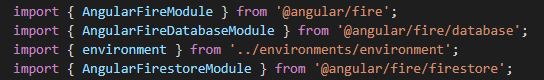
\includegraphics[scale=1]{./img/firebaseImports.png}
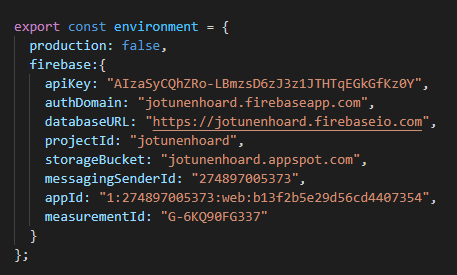
\includegraphics[scale=1]{./img/environment.png}

\subsection{Database Model: JotunenHoard}
JotunenHoard is the name of the Cloud Firestore database used in this project. It has three main Collections at the base of the project. These are 'Forums', 'Messaging' and 'Users'.
\subsubsection{Database Model}
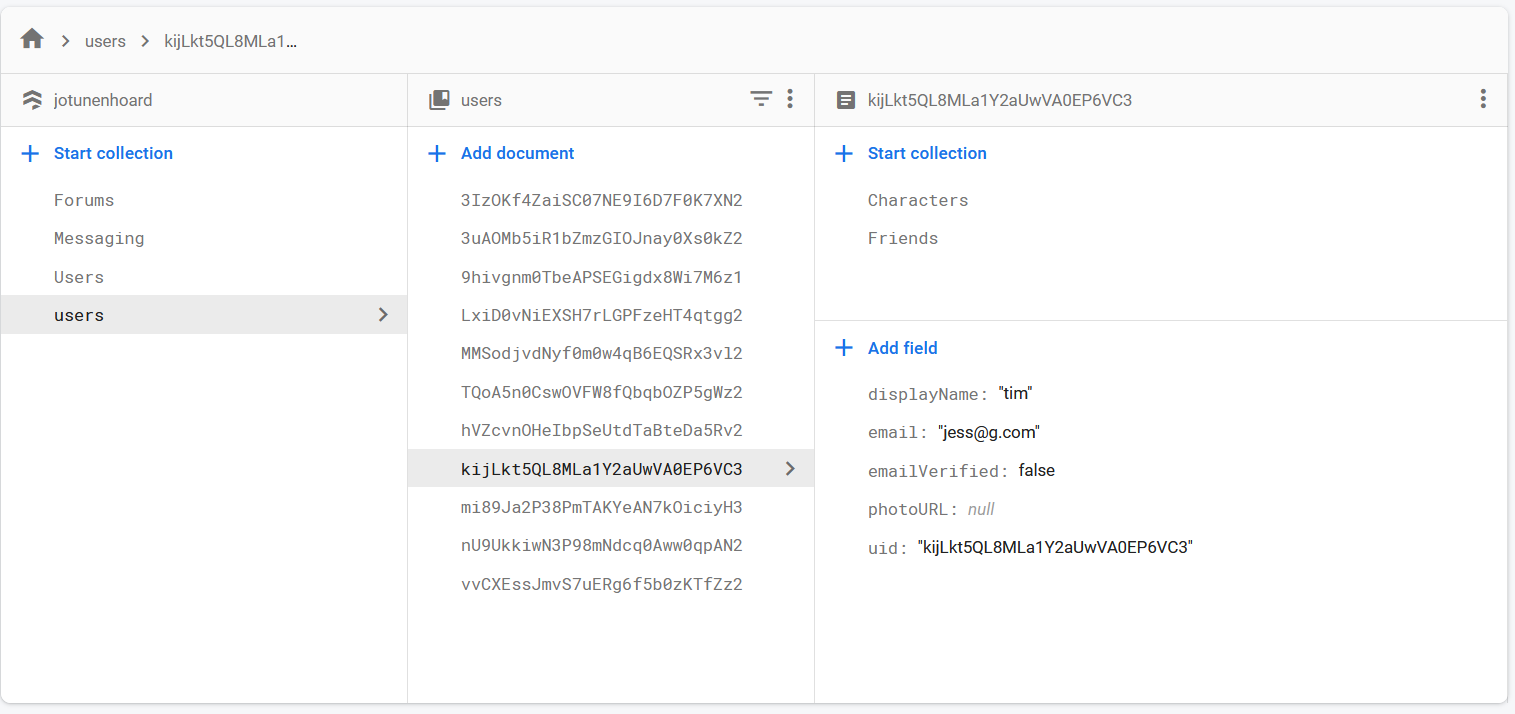
\includegraphics[scale=0.3]{./img/Database.png}
\subsubsection{Database UML:}
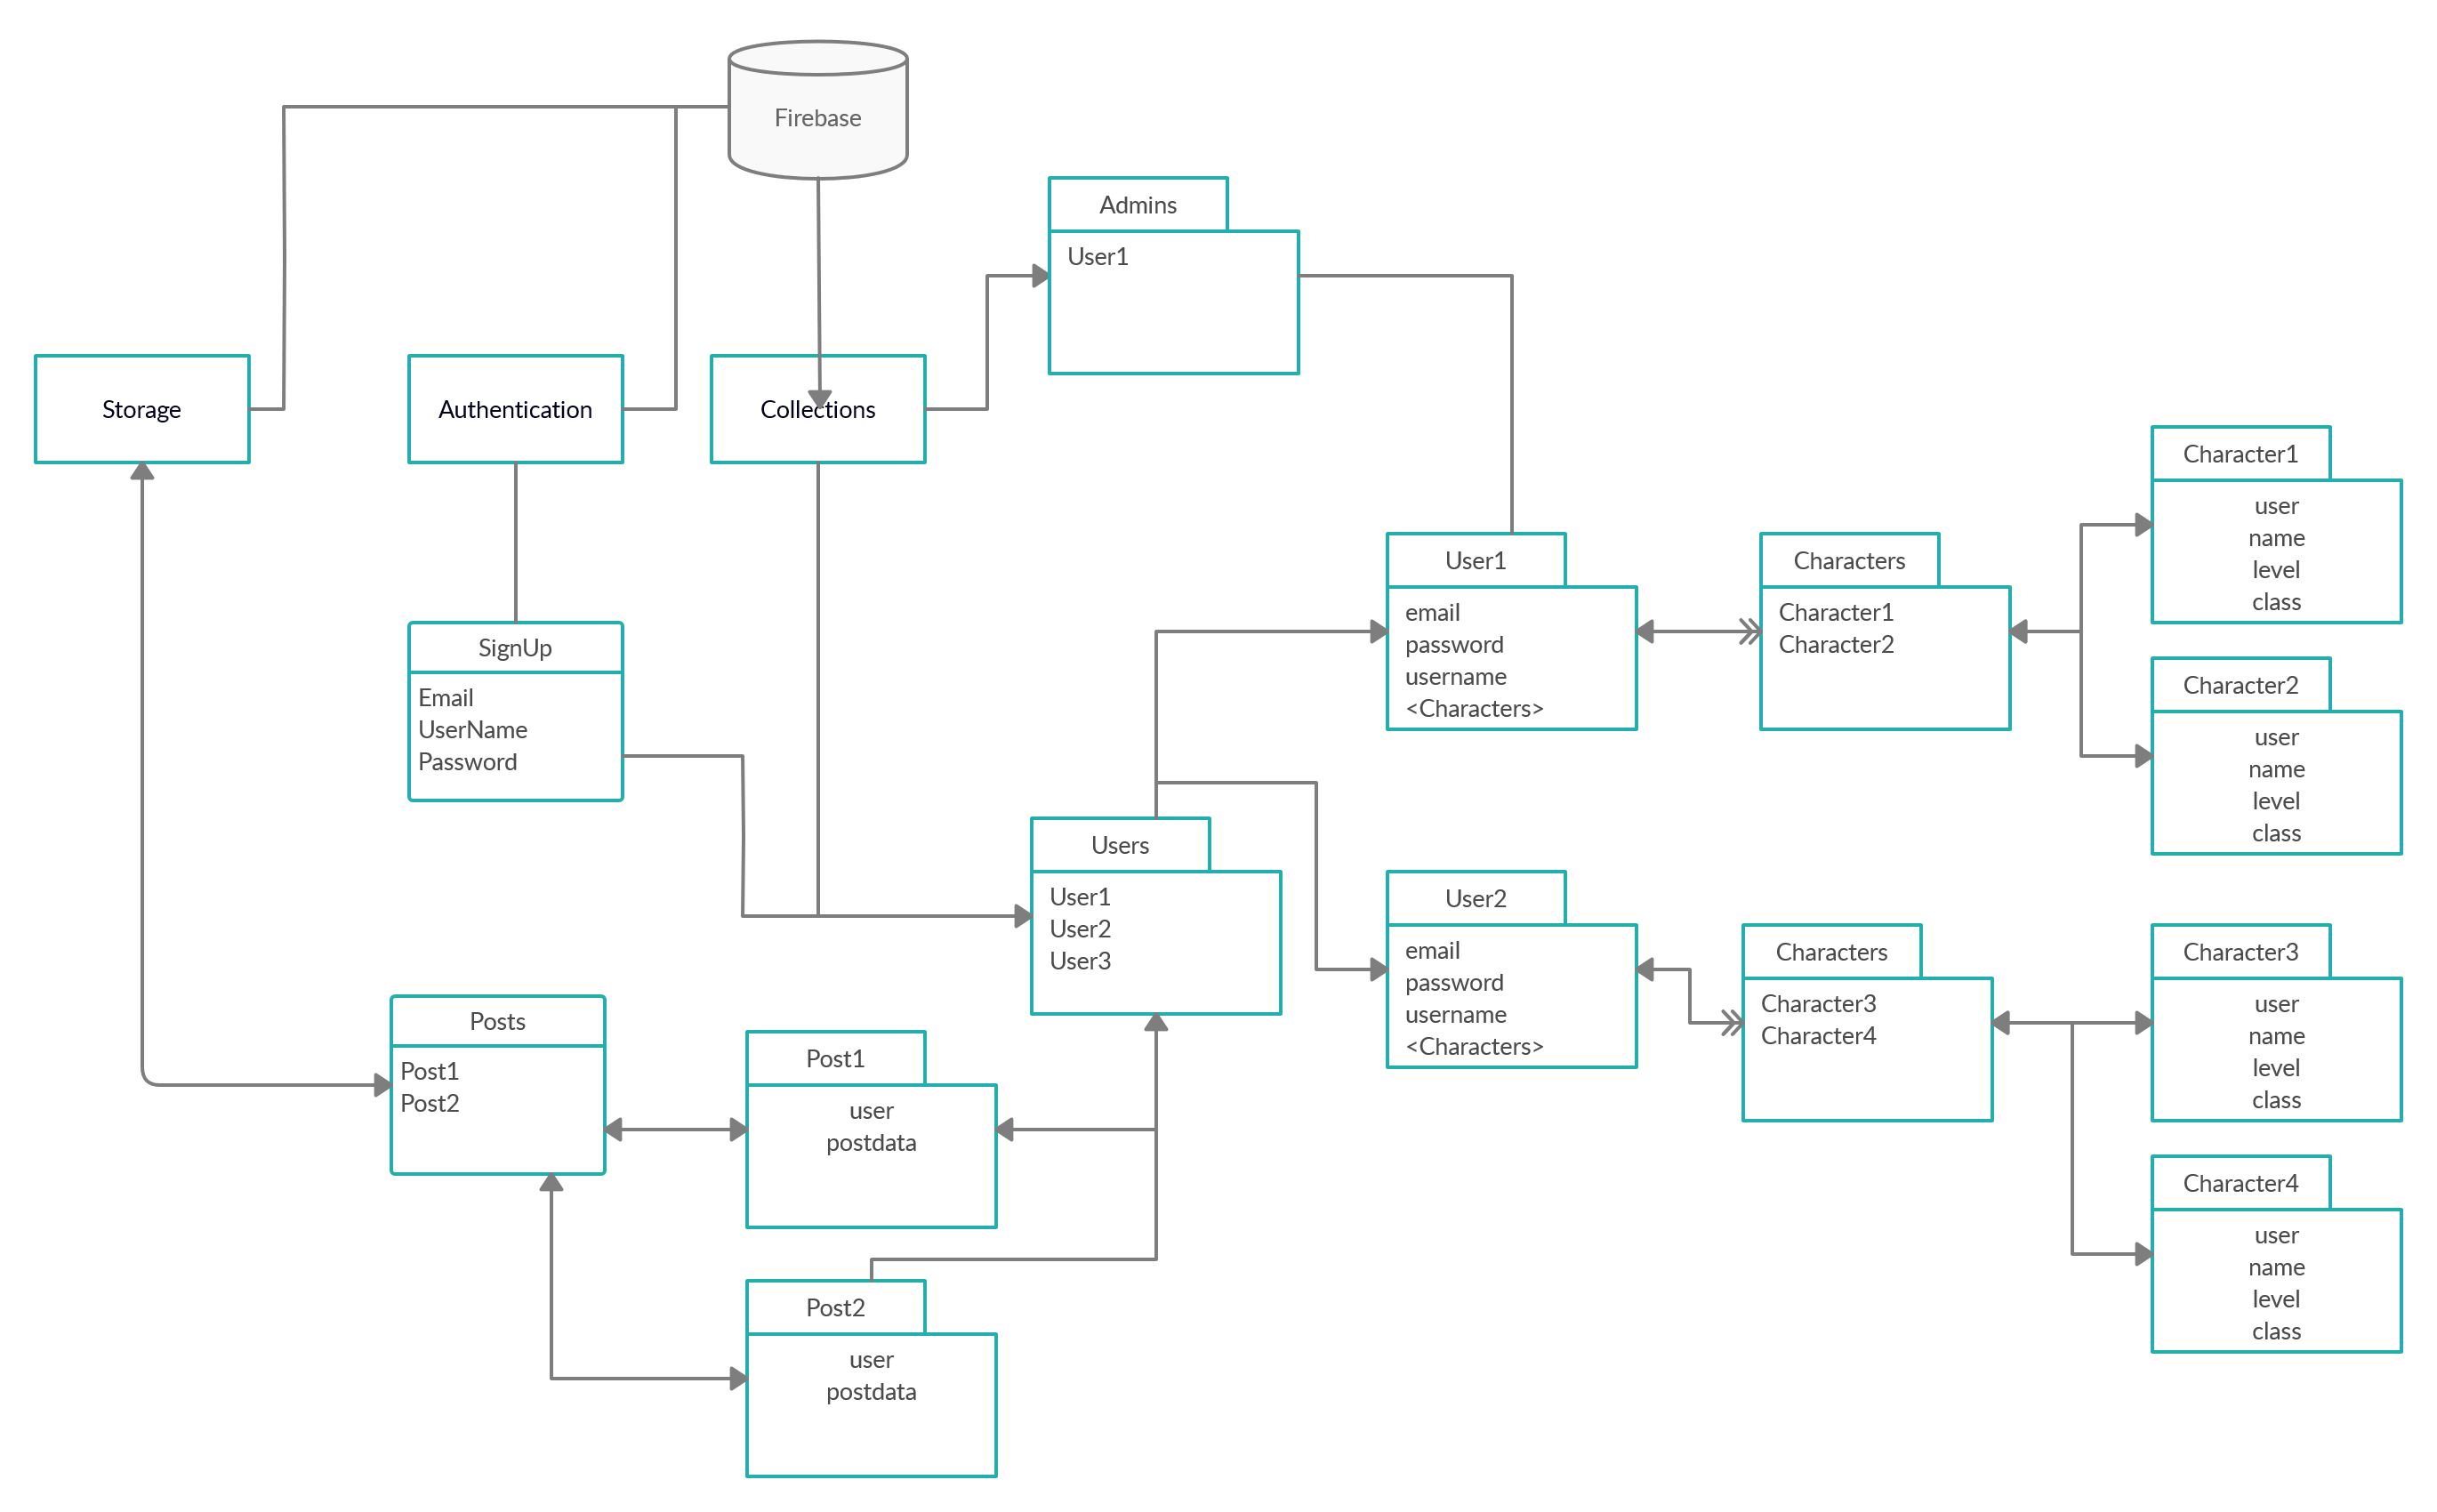
\includegraphics[scale=0.1]{./img/FirebaseUML.png}

\subsubsection{Collection: Users}
The Users collection is a collection of User Documents. Every Document contains field variables that store relevant information about the user and are added when it is create by calling the 'register()' method in  'fire-authentication.service'. It uses a User model predefined by firebase to store a users displayName, email and uid. Inside each document can be a Friends Collection and Characters Collection that are created once called from the project. These Collections Store documents of Characters the user has created and other users as well as the most recent message sent in a conversation.
\subsubsection{User Model:}
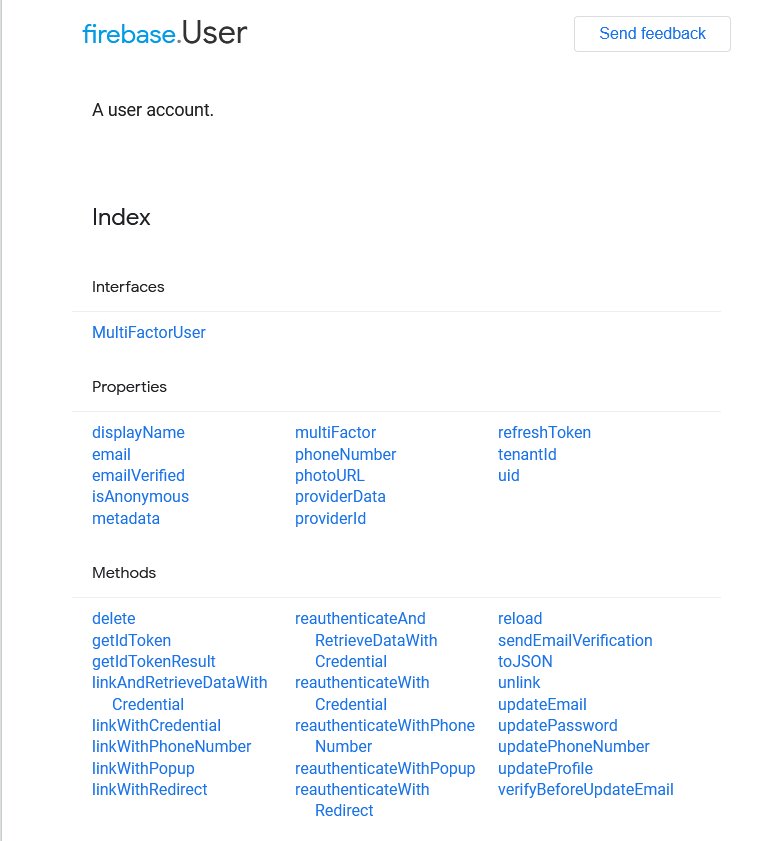
\includegraphics[scale=0.3]{./img/firebaseUser.png}
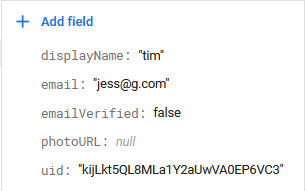
\includegraphics[scale=0.8]{./img/UserValues.png}
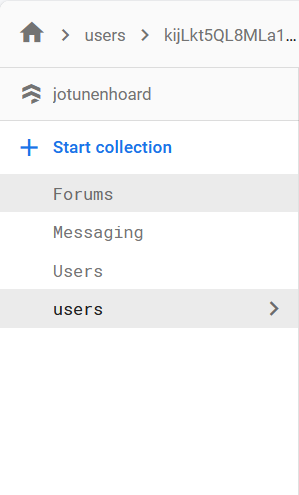
\includegraphics[scale=0.3]{./img/Collections.png}
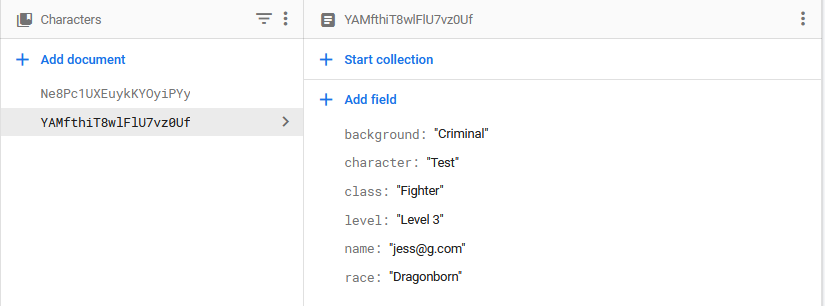
\includegraphics[scale=0.3]{./img/Characters.png}
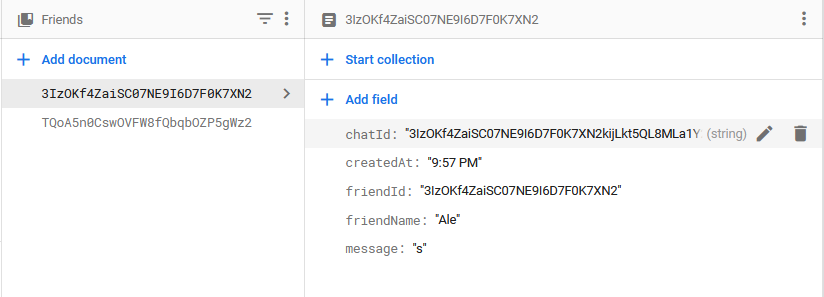
\includegraphics[scale=0.3]{./img/Friends.png}

\subsubsection{Collection: Messages}
The Messages collections contains a set of documents who's titles is a Unique ID generated by combining the unique ID of two users. In this document is the information of the latest message information saved and a collection of documents containing every individual Message sent in a conversation between two users. A message document contains the contents of the messages, the time it was sent, the IDs of the users involved and the chatId.
\subsubsection{Messages Collection Model:}
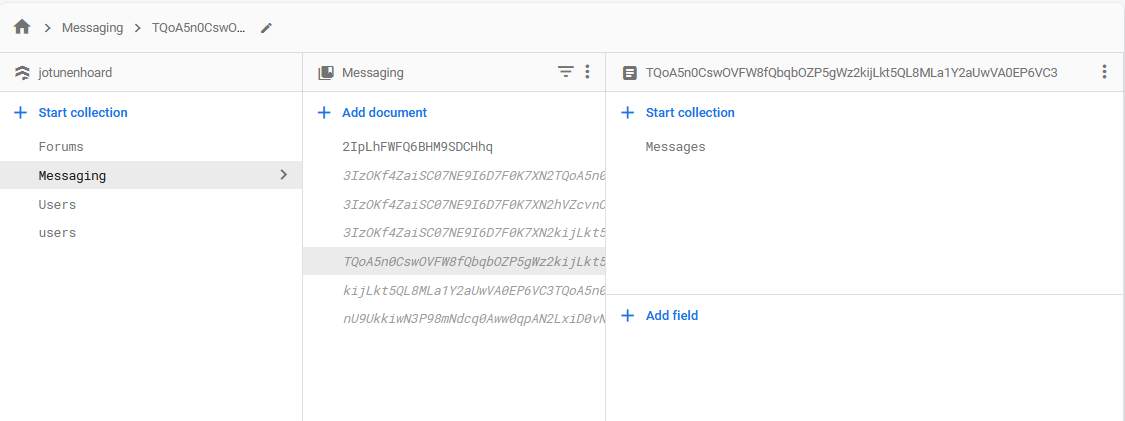
\includegraphics[scale=0.2]{./img/MessagingModel.png}
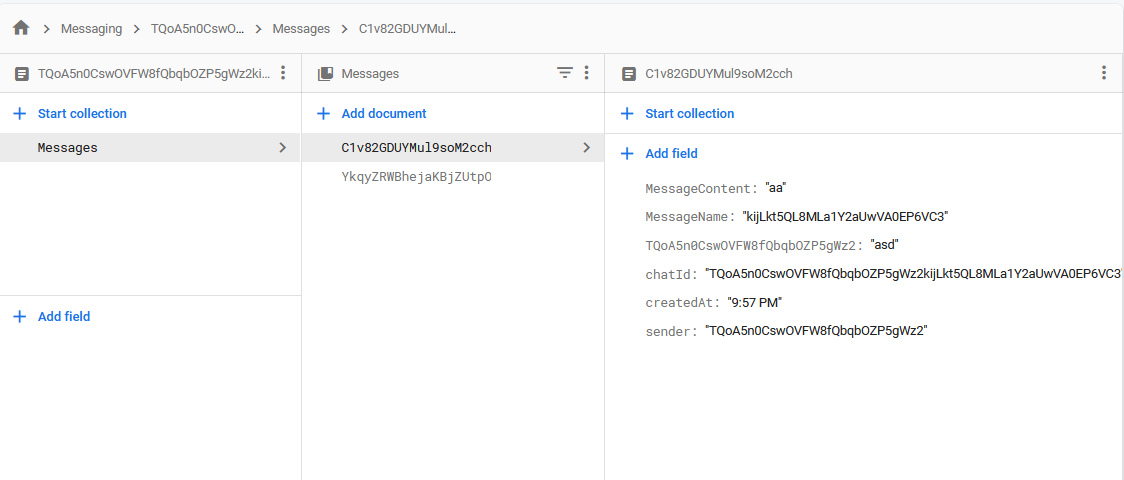
\includegraphics[scale=0.2]{./img/MessagingDocument.png}

\subsubsection{Collection: Forums}
The forums Collection contains a set of documents who's titles are uniquely generated by combining a users unique ID and the Title of the post. In these documents are the information and contents of the post, as well as a collection of Comments inside each which store all replies posted on a forum.
\subsubsection{Forums Collection Model:}
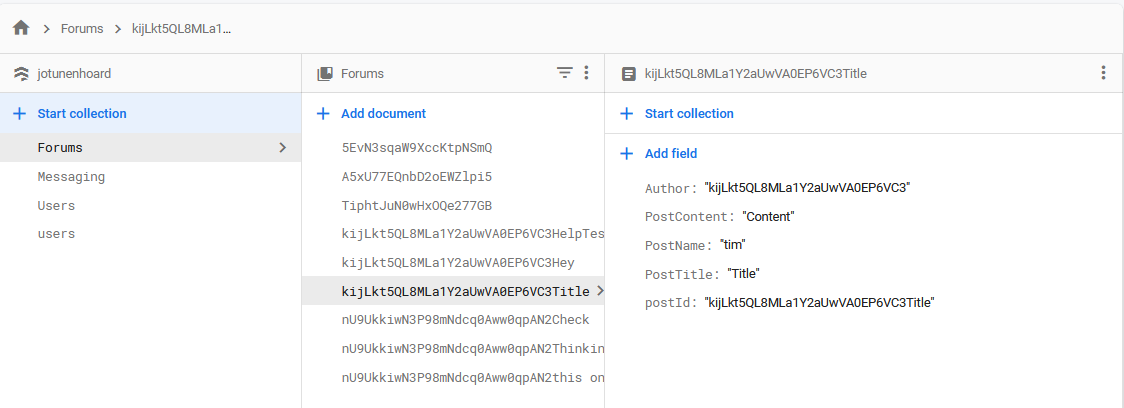
\includegraphics[scale=0.3]{./img/Forums.png}
\subsubsection{Firebase Rules:}
Firebase has a rules sections where you can manipulate the rules of the server. The rules on this server prevents all users who are not authenticated, will only allow permissions to read documents regardless of any other rules. After the account is authenticated the user has permissions where available.
\subsubsection{Firebase Rules Snippet:}
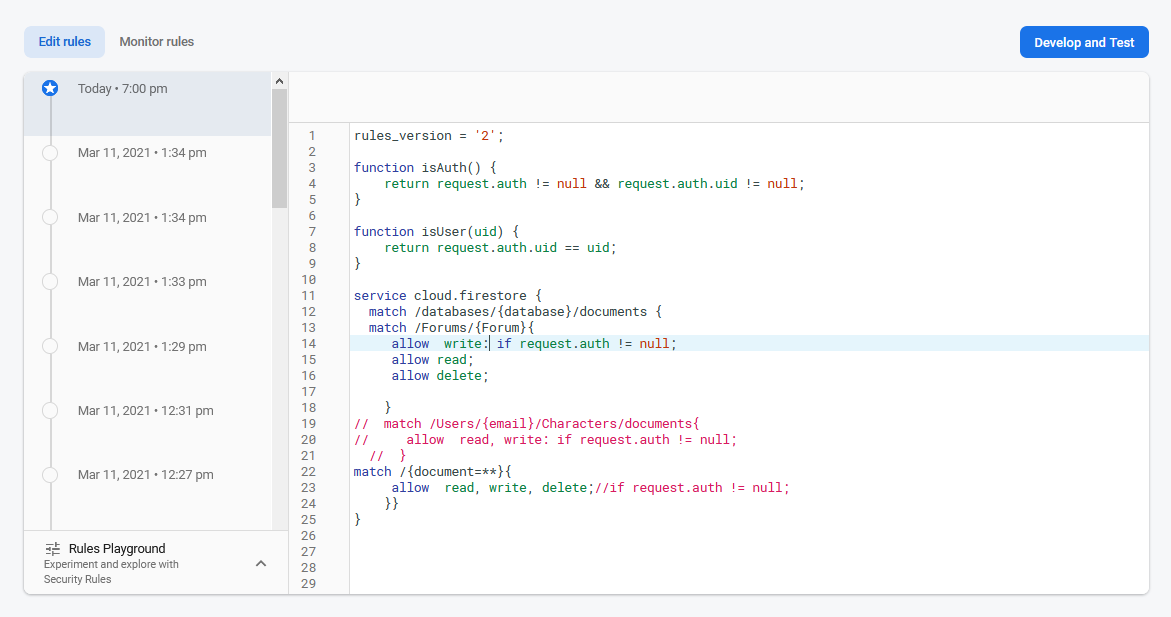
\includegraphics[scale=0.3]{./img/FirebaseRules.png}
\subsection{Authentication}
 which use the Angular Authentication method  this.afAuth.createUserWithEmailAndPassword(email, password)

\subsection{Sign Up Page}
This page prompts the user to register an account for the application. The user is prompted to fill in the Register User form, which includes the email address, password and username. Once all values are filled, the password is valid and the Sign Up button is clicked the Register() method is called from the fire-authentication.service which uses the firebase 'AngularFireAuth''s createUserWithEmailAndPassword(email, password) method, which checks if the user email is unique and creates a User document in the User/ collection. After it is authenticated the homepage is then loaded.
\\\\
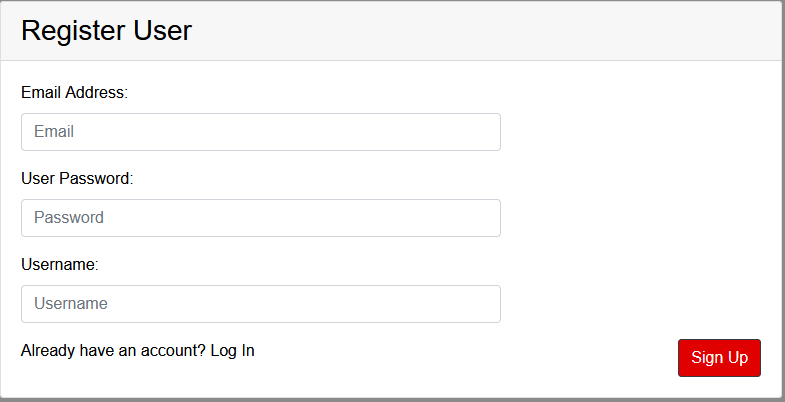
\includegraphics[scale=0.3]{./img/SignUpPage.png} 
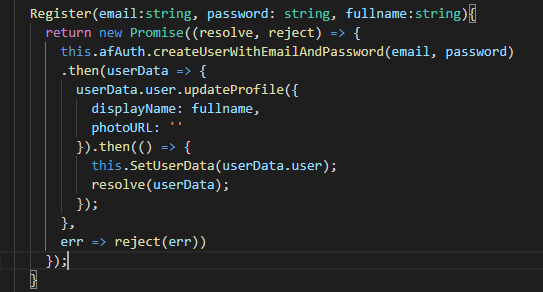
\includegraphics[scale=0.4]{./img/Register.png}\\
\subsection{Sign In Page}
The root-page redirects to the Sign In page, rather then the homepage if the user has not logged in yet. The user is prompted to fill  in a Sign In form. This forum is comprised of an email address and user password. Once the fields have been filled the 'Sign In' button is available and upon being clicked the 'SignIn()' method is called. It returns a value using 'AngularFireAuth's signInWithEmailAndPassword(email, password) and then maps the result and saves the user information to a constant variable called userState, if the password and email are valid. The homepage is then loaded. 
\\\\
The "Already have an account? Log in" option at the bottom of the form redirects the user to the Sign In page allowing them to log in with an account they have previously made.
\\\\
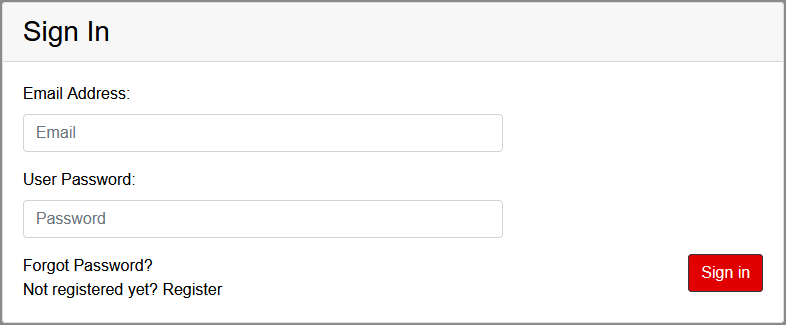
\includegraphics[scale=0.3]{./img/SignInPage.png} 
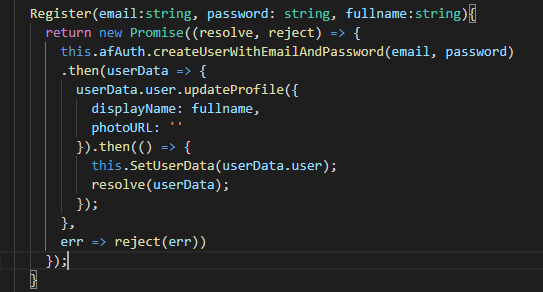
\includegraphics[scale=0.4]{./img/Register.png}\\

\subsection{Messages Page}
The Messaging Page's main functionality is to allow users to message other users and display their messages. At the top of the page the user is welcomed to the website and their username is displayed. There is a Message form present on the page that allows the user to input a users id and input the message into a text area that they wish to send. Once these are filled the user can then click the 'Send Message' button to send the message to the user by calling the CreateMessage() method. This adds the message to a record and calls the postMessage() method in the 'fire-authentication.service'. It calculates the current time and adds extra information to the post, such as the sender name. It calls the friendUpdateSender() and friendUpdateTarget to update the last messaged sent variable in the User/sampleuser/firends/samplefriend/lastMessage.\\\\
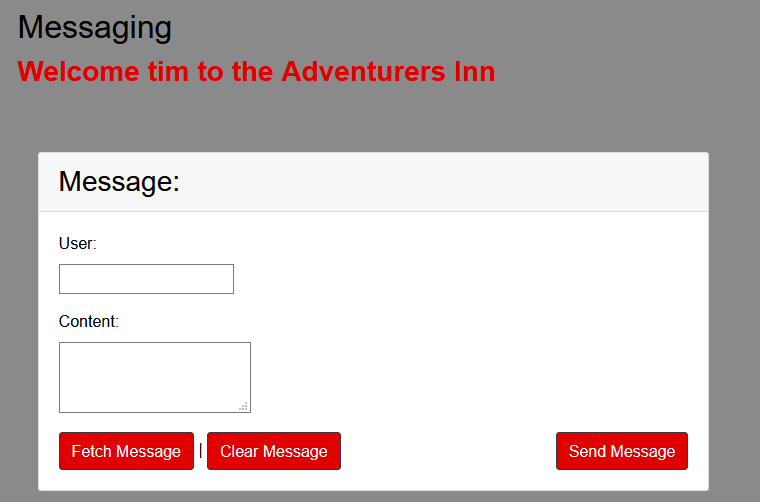
\includegraphics[scale=0.3]{./img/MessagingInput.png} 
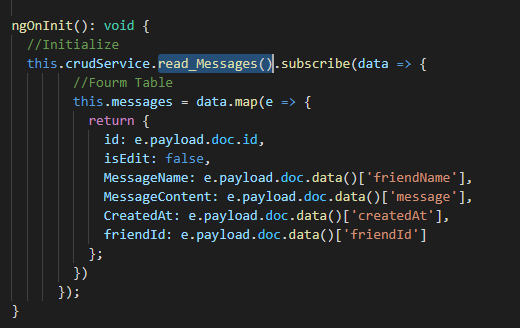
\includegraphics[scale=0.3]{./img/MessageMapping.png} 
\\\\
If the user has a message, the most recent message from each individual user is displayed. It does this by readMessages() method in 'fire-authentication.service'. It does this by mapping the result returned values from the snapshotChanges() method. Once clicked it loads a subpage where all messages can be displayed.
\\\\
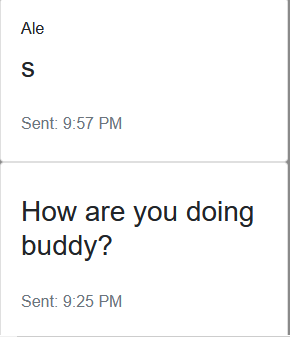
\includegraphics[scale=0.4]{./img/DisplayMessages.png}
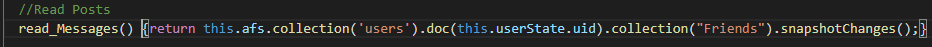
\includegraphics[scale=0.3]{./img/ReadMessage.png} 


\subsection{Forums Page}
The Forums Page is responsible for allowing the user to post to a forums about their individual campaigns using the  CreatePost() method. The  CreatePost() packages the input into a record object and then calls the postForum() method. This posts it to a forum where the forum Id is a combination of the user unique id and the post title. This might be the name of there party, campaign other whatever other topic they would like Other users of the application are then able to see these posts on the homepage and the forums page. The application then reads the posts from the collection Forums and displays them after mapping them by using the readForums() method.\\
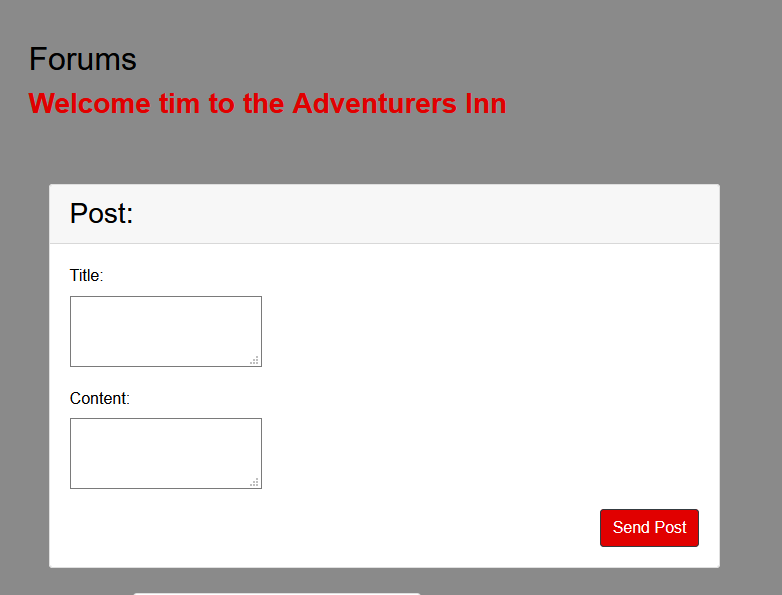
\includegraphics[scale=0.3]{./img/ForumInput.PNG} 
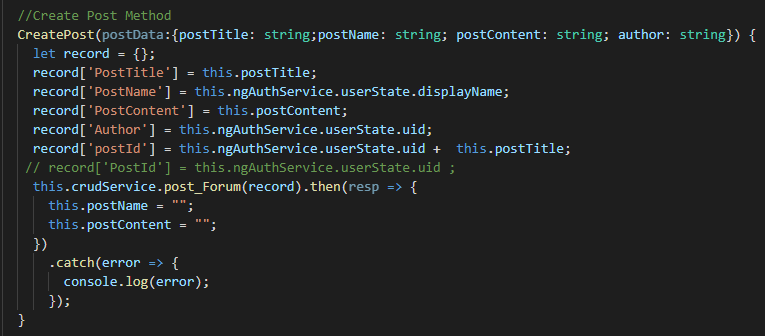
\includegraphics[scale=0.3]{./img/CreatePost.PNG}
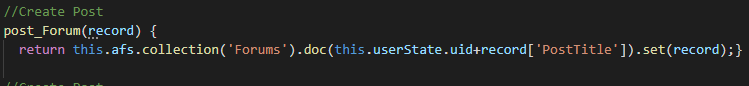
\includegraphics[scale=0.3]{./img/PostForum.PNG}
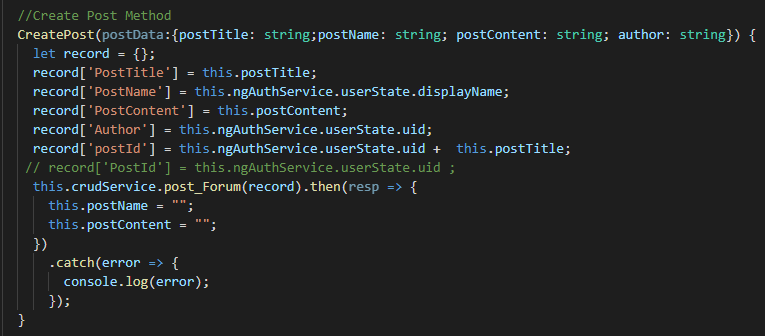
\includegraphics[scale=0.3]{./img/CreatePost.PNG}
At the top of the page the user is welcomed to the website and their username is displayed. \\
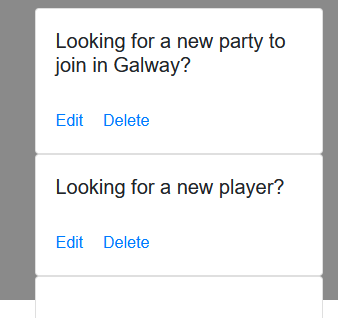
\includegraphics[scale=0.3]{./img/ForumsRead.png} \\
 They also have the option to write about the contents of the post if they wish, once they user has filled in their desired information they can press the "Send Post" button which will add the post the forums collection in the database. \\
 
 The user may then click on the title of a post to view it in entirely. Upon clicking the tile the postComponent page is loaded which saves the post details as a localStorage JSON object. The post then displays this information and then reads the forum by using the postId to access the data using the readPost().\\
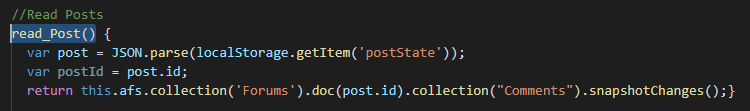
\includegraphics[scale=0.3]{./img/GetPost.png} \\

By mapping the documents in the forums/sampleForum/ collection, the application displays all comments and replies posted on the forums by other verified users. The users will be able to reply to these comments and eventually like and dislike individual posts and comments.\\
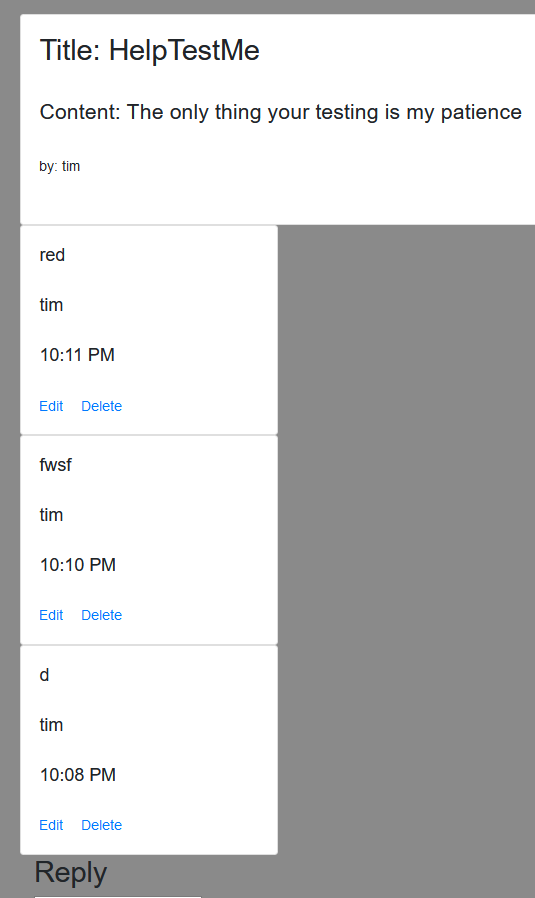
\includegraphics[scale=0.3]{./img/Post.png} 
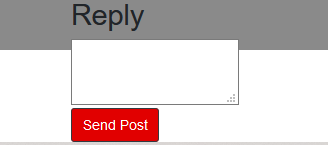
\includegraphics[scale=0.3]{./img/Reply.png} \\

\subsection{HomePage}
The homepage is where the user will be automatically redirected to, after signing up or logging in to the application. It displays the forums post and will eventually filter by date, popularity and type of post. This feature is not fully implemented yet.
\subsection{App.Module}
This is where the imports of the project are managed and added to the project.\\
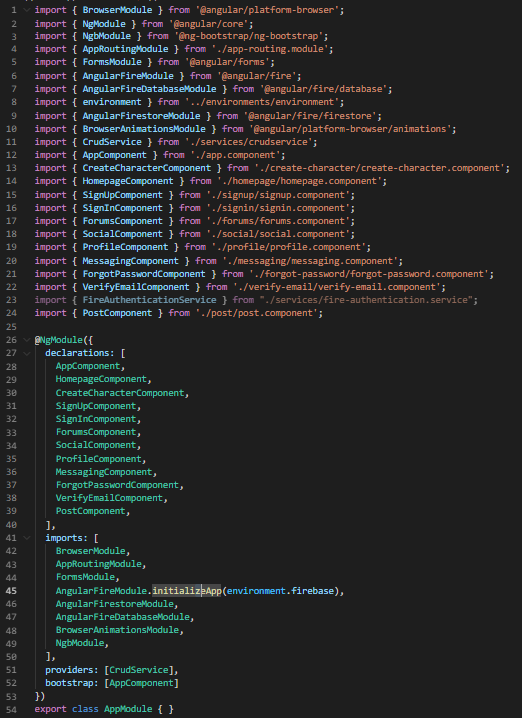
\includegraphics[scale=0.3]{./img/Imports.png} \\
\subsection{Groups Page}
This page is a page to manage the different groups the user is a part of. This has yet to be fully implemented.
\subsection{My Profile Page}
This page displays the users information at the top. This allows the user to give his Unique ID to another player if they want to add them to their friends list. It has a Sign Out button which allows the user to log out of their profile. There are two buttons to navigate to the Create character page and the Messaging page respectively. Below this is a card that displays the user's character which upon clicking loads a character details page. The user is able to quickly edit their own characters here.\\

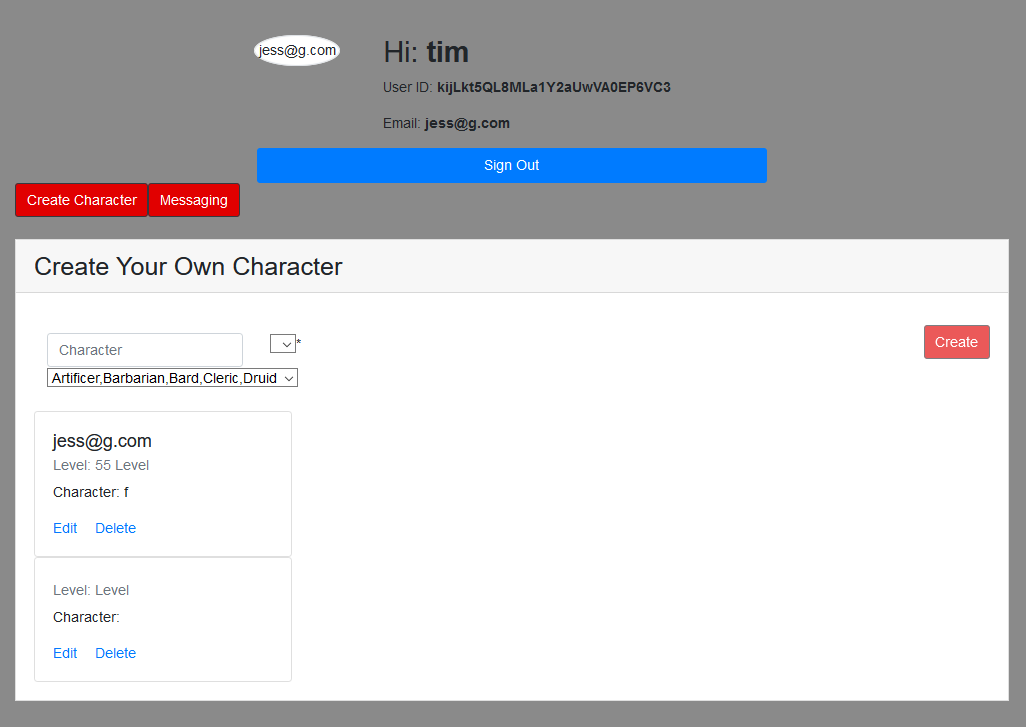
\includegraphics[scale=0.3]{./img/Profile.png} \\
\subsection{Create Character}
This page allows the user to create a new character based on the rules for Dungeons and Dragons 5th Edition. The user must then input there character details including their character names, level, , Race, Class and Background. It used the  CreateRecord() method which maps the information into a record and then calls the createNewCharacter() method from the 'fire-authentication.service'. This pushed the record to the database and creates a character document in the collection Users/sampleUser/Characters/.\\
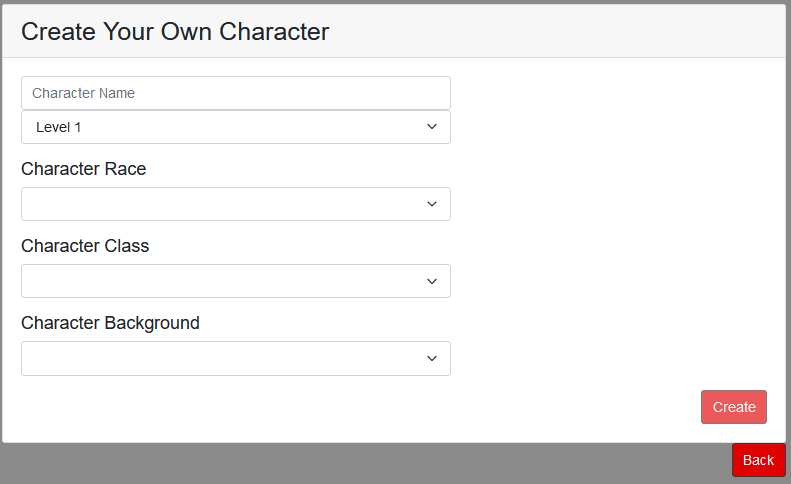
\includegraphics[scale=0.3]{./img/CreateCharacter.png} \\
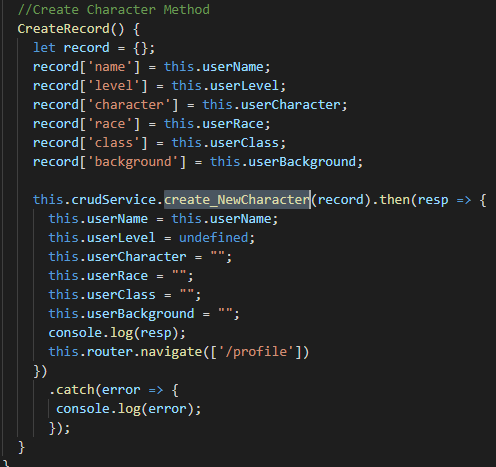
\includegraphics[scale=0.3]{./img/CreateRecord.png} \\
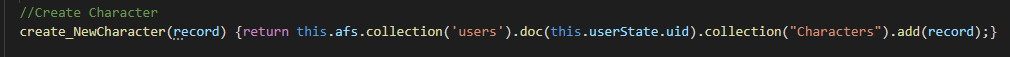
\includegraphics[scale=0.3]{./img/CreateNewCharacter.png} \\

\section{Container}
Containerized software was used to make a container image to package the code and dependency of the application, so that it could be easily and reliably be form the environment on our local machines (Windows 10) to the environment on the virtual machine (Ubuntu).  This meant that if the application need to be run on a environment there would not be any unnecessary complication.

\subsection{Docker}
For the purpose of this project, Docker was the containerized software used.  In this project Docker creates a Container image of the application at runtime, allow the application to run on both of the environments being used in the project.  Docker was executed using the Standard Docker CLI interface. The Dockerfile script was used for creating a containerize image of the application at runtime.  This could then be used to run the application.
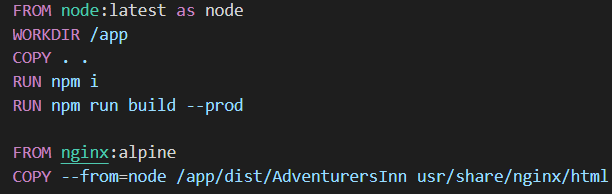
\includegraphics[scale=0.3]{./img/docker.PNG}

\section{Cloud Storage}
The cloud platform used for the purpose of this project was Microsoft Azure.  The cloud platform was used to extract the running of the application away for our personal machine, the reasoning behind this was that it would not be dependent on personal computers of WiFi connections.  

\subsection{Azure Virtual Machine}
The Azure Virtual Machine Azure was a Ubuntu based server-side virtual machine used for deploying and hosting the application.